\documentclass[12pt]{article}
\usepackage[english]{babel}
\usepackage[utf8x]{inputenc}
\usepackage{amsmath}
\usepackage{graphicx}
\usepackage{tabularx, makecell}
\usepackage[dvipsnames]{xcolor}
\usepackage{listings}
\usepackage{alloy-style}


\def \thisDocVersion {\texttt{v.0}}

% TODO finish section 1

% === RASD ===
%The Requirements analysis and specification document (RASD) contains the description of the scenarios, the use cases that describe them, and the models describing requirements and specification for the problem under consideration. You are to use a suitable mix of natural language, UML, and Alloy. UML and Alloy MUST be part of the documentation. You must also show that you used the Alloy tool for analysis, by reporting the models you obtained by using it. Of course, the initial written problem statement we provide suffers from the typical drawbacks of natural language descriptions: it is informal, incomplete, uses different terms for the same concepts, and the like. You may choose to solve the incompleteness and ambiguity as you wish, but be careful to clearly document the choices you make and the corresponding rationale. You will also include in the document information on the number of hours each group member has worked towards the fulfillment of this deadline. As a reference structure for your document, you should refer to the one reported below that is derived from the one suggested by IEEE. Please include in the document information about the effort spent by each group member for completing this document.

% === TrackMe ===
%TrackMe is a company that wants to develop a software-based service allowing third parties to monitor the location and health status of individuals. This service is called Data4Help. The service supports the registration of individuals who, by registering, agree that TrackMe acquires their data (data acquisition can happen through smartwatches or similar devices). Also, it supports the registration of third parties.
%After registration, these third parties can request:
%\begin{itemize}
%  \item Access to the data of some specific individuals (we can assume, for instance, that they know an individual by his/her social security number or fiscal code in Italy). In this case, TrackMe passes the request to the specific individuals who can accept or refuse it
%  \item Access to anonymized data of groups of individuals (for instance, all those living in a certain geographical area, all those of a specific age range, etc.). These requests are handled directly by TrackMe that approves them if it is able to properly anonymize the requested data. For instance, if the third party is asking for data about 10-year-old children living in a certain street in Milano and the number of these children is two, then the third party could be able to derive their identity simply having people monitoring the residents of the street between 8.00 and 9.00 when kids go to school. Then, to avoid this risk and the possibility of a misuse of data, TrackMe will not accept the request. For simplicity, we assume that TrackMe will accept any request for which the number of individuals whose data satisfy the request is higher than 1000
%\end{itemize}
%As soon as a request for data is approved, TrackMe makes the previously saved data available to the third party. Also, it allows the third party to subscribe to new data and to receive them as soon as they are produced.
%Imagine now that, after some time, TrackMe realizes that a good part of its third-party customers wants to use the data acquired through Data4Help to offer a personalized and non-intrusive SOS service to elderly people. Therefore, TrackMe decides to build a new service, called AutomatedSOS, on top of Data4Help. AutomatedSOS monitors the health status of the subscribed customers and, when such parameters are below certain thresholds, sends to the location of the customer an ambulance, guaranteeing a reaction time of less than 5 seconds from the time the parameters are below the threshold.

\begin{document}
\documentclass[../DD0.tex]{subfiles}
\begin{document}

\begin{titlepage}
  \newcommand{\HRule}{\rule{\linewidth}{0.5mm}}
  \center
  \includegraphics[width=140pt]{\fetchImg{polimi.png}}\\[1cm]
  \textsc{\LARGE Politecnico di Milano}\\[1cm]
  \textsc{\Large Master's Degree in \\Computer Science and Engineering}\\[0.5cm]
  \textsc{\large Software Engineering 2}\\[0.5cm]
  \HRule \\[0.4cm]
  { \huge \bfseries TrackMe\\[0.4cm] Design Document }\\[0.4cm]

  \HRule \\[1cm]
  \begin{minipage}{0.4\textwidth}
  \begin{flushleft} \large
  \emph{Authors}\\
  Alberto \textsc{Archetti}

  Fabio \textsc{Carminati}
  \end{flushleft}
  \end{minipage}
  ~
  \begin{minipage}{0.4\textwidth}
  \begin{flushright} \large
  \emph{Reference professor} \\
  Elisabetta \textsc{Di Nitto}
  \end{flushright}
  \end{minipage}\\[1cm]
  {\large \thisDocVersion\ - \today}\\[1cm]
  \vfill
\end{titlepage}
\end{document}

\clearpage
\pagenumbering{gobble}
\nonumber
\tableofcontents
\clearpage
\pagenumbering{arabic}
\clearpage
\documentclass[../DD0.tex]{subfiles}

\newcommand{\addRevision}[2]{\texttt{v.#1} & #2 \\ \hline}

\begin{document}

\section{Introduction}
\label{sec:intro}

  \subsection{Purpose}
  \label{sec:purpose}

    TrackMe wants to develop a software-based service that allows individual users to collect health data, called \texttt{Data4Help}. This data can be retrived from the system and visualized according to different filters by a user interface. \\
    The system allows third parties registration. Third parties can request access to users'collected data in two ways:

    \begin{description}
      \item [\textbf{Single user data}] After a third party makes a request to the system for a single user data sharing, by providing  user's fiscal code, the system asks the user for authorization; if positively provided, the third party is granted access to the user's data
      \item [\textbf{Amonymous group data}] Third parties can be interested in big amounts of data, but not in who are the people providing it; the system, once the request is sent by the third party, checks if the data can be effectively anonymized (it must find at least 1000 people that can provide data matching the third party request's filters) and, if positively evaluated, grants access to the anonymized data to the third party
    \end{description}

    Third parties can subscribe to new data and receive it as soon as it is collected by the system.

    Another service that TrackMe wants to develop is \texttt{AutomatedSOS}, built on \texttt{Data4Help}. This service analyzes users'data and calls a SOS whenever data exceedes the basic health parameters. For this particular purpose, system performance will be a critical aspect to be taken into account, because even the slightest delay matters in critical health situations.

    We will list the project \textbf{goals}, described in the RASD document:
    \begin{description}
      \item[\texttt{G.U1}] Users can collect, store and manage their health data
      \item[\texttt{G.U2}] Users can choose to have their health monitored; if their health is critical, an ambulance will be dispatched
      \item[\texttt{G.T1}] Third parties can ask single users for their health data sharing
      \item[\texttt{G.T2}] Third parties can request access to anonymized data that comes from groups of people
      \item[\texttt{G.T3}] Third parties can subscribe to new data and receive it as soon as it is produced
    \end{description}

  \subsection{Scope}
  \label{sec:scope}

    \subsubsection{World}

      Our \textit{world} is composed of two main types of actors: \textit{users} and \textit{third parties}. Users are interested in monitoring their health parameters and third parties are interested in developing services or researches that exploit data gathered from the users. \texttt{Data4Help} is the service that acts as a bridge between these actors'needs. \\
      Phenomena that occur in the \textit{world} and are related to our application domain are
      \begin{itemize}
        \item physical conditions of the users
        \item third parties'projects, researches and interests
        \item ambulances dispatched by the SOS system
      \end{itemize}
      These phenomena exist in the \textit{world}, but cannot be observerd directly by our system.

    \subsubsection{Shared phenomena}
    \label{sec:sharedp}

      In order to communicate with the \textit{world}, our system needs to share some aspects with it. We will list the aspects controlled by the world, but observable by the machine:
      \begin{description}
        \item[\texttt{S.1}] physical parameters of the users, gathered through sensors on wereable devices
        \item[\texttt{S.2}] third parties requests to the system for the data they need
        \item[\texttt{S.3}] users'location, acquired through GPS signals
      \end{description}
      On the other hand, the aspects that occur in the machine, but are observable by the world are
      \begin{description}
        \item[\texttt{S.4}] interfaces that organize the gathered data that can be filtered according to time or type of data
        \item[\texttt{S.5}] messages for the SOS system, that are sent in case of critical health of a user
        \item[\texttt{S.6}] payment requests
      \end{description}

  \subsection{Definitions}
  \label{sec:definitions}

    \begin{description}
      \item[Data] Quantitative variables concerning health parameters
      \begin{description}
        \item[Aggregate data] See \textit{DataSet}
        \item[Anonymous data] \textit{data entry} that doesn't contain information about the user from which it was produced; a \textit{data set} is said to be anonymized if it contains only anonymous \textit{data entries} and its cardinality is greater or equal than 1000
        \item[Data entry] Tuple that corresponds to the user's parameters in a particular moment
        \item[Data set] Set of \textit{data entries}; depending on the context, it can identify a set of entries all belonging to a single user or or a set of anonymous entries belonging to more that 1000 users; a \textit{data set}, among all \textit{data} that the system is storing, can be identified and constructed according to the filters of a third party request
      \end{description}
      \item[Request] Third parties can ask the system for some data sharing through requests; requests are encoded through filling a form; the system, provided that the request is satisfiable, grants the third party access to the requested data
      \item[Third party] Actor interested in collecting data from a single user or from an anonymous group of users
      \item[Threshold] Numerical values related to a particular health parameter; they act as boundaries between the domain of critical health status and normal health status
      \item[User] Actor interested in his/her health data collecting and managing; a user can also be interested in automating SOS calls whenever his health status becomes critical
    \end{description}

    Some of these definitions may already be present and further explained in the RASD document.

  \subsection{Acronyms and abbreviations}
  \label{sec:acronyms}

    \begin{description}
      \item[API] Application Programming Interface
      \item[DBMS] Database Management System
      \item[Data] Whenever the context refers to generic groups of \textit{data entries}, the terms \textit{data} and \textit{data set} are interchangeable
      \item[System] Software product that TrackMe wants to develop; can be interchanged with \textit{S2B}
      \item[S2B] Software To Be
    \end{description}

  \subsection{Revision history}
  \label{sec:revhistory}

    \begin{table}[!h]
      \begin{tabular}{|c|l|}
        \hline
        \textbf{Version}  & \textbf{Log} \\ \hline
        \addRevision{0}{DD first draft}
      \end{tabular}
    \end{table}

  \subsection{Document structure}
  \label{sec:docstructure}

  This document describes architecture and design of \texttt{Data4Help} and \texttt{AutomatedSOS} systems. The description will start with a top-down approach, in order to make the reader familiar with the overall structure; a bottom-up approach will then be adopted, in order to describe components in a isolated way. This document is devided in
  \begin{itemize}
    \item Section~\ref{sec:intro} is a brief introduction on the project to be developed in order to make this document self-contained
    \item Section~\ref{sec:arcdes} describes the high-level architecture (high-level components, their interation, runtime views and architextural decisions)
    \item Section~\ref{sec:ui} provides an overview on how the user interface will look like
    \item Section~\ref{sec:req} contains mapping between software requirements, described in the RASD document, and design elements
    \item Section~\ref{sec:imp} identifies the order in which subcomponents will be implemented, integrated and tested
    \item Section~\ref{sec:effort} lists the work sessions that drove this document's development, ordered by date, as the hour counter of effort spent by each group member
  \end{itemize}

\end{document}

\clearpage
\section{Overall description}
\label{sec:overdesc}

  \subsection{Product perspective}

    \texttt{Data4Help} is a service oriented to data acquisition and data sharing. Its software nature rises the necessity to combine it with another service able to directly retrive raw data from the \textit{world}. Today we can find for sale multiple wearables  that can acquire data from users and make it readable from software side. \texttt{Data4Help} users should already own these devices in order to exploit the data acquisition functionality (Section~\ref{sec:sharedp}: \textbf{\texttt{S.1}}). Once the user registered to the service, its interface will gather the last data collected and organize it in a chart view, that can be filtered by data or type and rendered by the user interface (Section~\ref{sec:sharedp}: \textbf{\texttt{S.4}}; Section~\ref{sec:userinterfaces}).

    It is mandatory for the user's wearable to provide a GPS signal, if the user wants to apply to the \texttt{AutomatedSOS} service. GPS will be used to track the user's location in case of health danger and the signal will be shared to the SOS service that already exists in the \textit{world} (Section~\ref{sec:sharedp}: \textbf{\texttt{S.3}}, \textbf{\texttt{S.5}}). This SOS service accepts messages that contain the GPS location of the person in health danger and an emergency log that \texttt{AutomatedSOS} generates from the acquired data. The log explains the suspected health danger and the data that passed the defined thresholds.
    % TODO check the consistency of this in the future

    Third party organization are interested in data gathering. In order to allow them to make requests for specific types of data, \texttt{Data4Help} provides a user interface that is in charge of composing their request, to make it understendable by the software (Section~\ref{sec:sharedp}: \textbf{\texttt{S.2}}; Section~\ref{sec:userinterfaces}). The interface provides all the possible options that the third party can compose in order to provide the closest data request to its needs.
    % TODO add UML diagrams
    % TODO add informal domain assumptions

  \subsection{Product functions}

    Here we present the major functions that our product will offer. Some of them will entirely be handled internally by our system, but for others it will rely on external services. In the latter case, we will specify that the system will not directly provide the service and we will add example systems that already exist in the \textit{world}, in order to guarantee the feasibility of the functions.

    \subsubsection{Profile management}

      The system will provide a registration form at which users and third parties can apply. Once registered, they will have a uniquely identifiable account, provided the requested information for its creation (see Table~\ref{tab:login}). Once the account has been successfully created, its owner can exploit the system's functionalities.

      Note that accounts for users and third parties must be distinguishable from the system perspective, as it should offer different functionalities to different account types, in order to reflect the account owners'needs.

      \begin{table}[h!]
        \centering
        \begin{tabularx}{\linewidth}{|c|X|X|}
          \hline
          \textbf{Account type} & \textbf{Required information}                                       & \textbf{Optional information}                                                   \\ \hline
          User                  & \textit{email, password, fiscal code, date of birth, weight, height}             & \textit{social status, address, hours of work per day, hours of sport per week} \\ \hline
          Third party           & \textit{email, password, third party name, third party description} & \textit{website, research interests}                                            \\ \hline
        \end{tabularx}
        \caption{Example of login form information}
        \label{tab:login}
      \end{table}

    \subsubsection{Data gathering}

      Data gathering is exploited through physical wearables that users wear and that can communicate with our software by API calls (ex. Google Fit API \cite{googlefitapi}). Data entries are identified with a timestamp and the owner user.

      Collected data types depend on wearables. For example, the most common sensors for health parameters that we find on smart clothing \cite{sensors} are pulse, body temperature, electrocardiogram, myocardial and blood oxygen.

      Data type handling should be implemented in a flexible and extensible way in the system, because wearables technologies change rapidly and our software should adapt in the least invasive way possible.

    \subsubsection{Data sharing}

      \texttt{Data4Help} relies on an internal database for data storage. Once data has just been added to the system, only the user that produced it will have access. Data sharing is exploited by granting access to the stored data to third parties, if their requests have been accepted.

      Third party requests are encoded in the system by filling a form that contains information like Table~\ref{tab:tprequest}. They can be accepted or rejected. In the former case the third party is granted access to the data, while in the latter it is not granted access.

      \begin{table}[h!]
        \centering
        \begin{tabularx}{\linewidth}{|l|X|X|}
          \hline
          \textbf{Request type} & \textbf{Accept condition}                                               & \textbf{Filters}                                                                                                                           \\ \hline
          Single-user           & Target user should accept the request through his/her account                                   & \textit{fiscal code of target user, from-date, to-date, data types (weight, heart rate, etc.), time granularity (seconds, minutes, hours)} \\ \hline
          Anonymous-group       & Every user should have accepted the automatic sharing of requested data & \textit{size, from-date, to-date, data types (weight, heart rate, etc.), user characteristics (age interval, weight interval, etc.)}       \\ \hline
        \end{tabularx}
        \caption{Example of third party request form}
        \label{tab:tprequest}
      \end{table}

    \subsubsection{Data management}

      Once a user collected some data, he/she can organize it by changing the view options in the user interface. These options depend on the device the user is working on, but will always provide basic filters such as time interval or data type. Once filters have been selected by the user, the graphical interface will render a chart that organizes collected data according to them (see Section~\ref{sec:userinterfaces}).
      % TODO maybe add something here on third parties

    \subsubsection{Payment handling}

      Payment will entirely be handled from an external software system that should
      \begin{itemize}
        \item initialize payment processes
        \item check if the payment is feasible and, if not, notify to our system
        \item handle the payment operation
        \item notify to our system if the operation has concluded correctly, otherwise notify the error occurred
      \end{itemize}
      There are plenty of payment handlers that exist in our \textit{world} and can be paired to our system (ex. PayPal API \cite{paypal}).

    \subsubsection{SOS handling}

      This function is heavily dependant on the country in which the SOS will be handled. Our system will only communicate to the emergency service that already exists in the \textit{world} through automatic API calls (ex. RapidSOS Emergency system for US \cite{sos}).

      Calls to SOS are handled by \texttt{AutomatedSOS} that signals users GPS position and health status feedback. Calls occur, if the user previously subscribed to \texttt{AutomatedSOS}, when his/her health parameters are below certain thresholds. The time between health danger detection and emergency call must be less than 5 seconds.

  \subsection{User characteristics}

    The following list contains the actors that are involved in the system functions:

      \begin{description}
        \item [User] Person interested in the \texttt{Data4Help} \textbf{data management} service; he/she is required to register to the \texttt{Data4Help} service in order to exploit its functionalities; he/she can also apply to the \texttt{AutomatedSOS} service; every user owns an appropriate device for \texttt{Data4Help} acquisition service that can monitor at least heartbeat and GPS location \\
        % TODO occhio all'assunzione qua sopra
        ex. \textit{an athlet that wants to monitor his/her physical status during sport activity, an old person that suffers from heart diseases or a sedentary worker that wants to keep track of his health parameters in the working hours}
        \item [Third Party] Entity interested in the \texttt{Data4Help} \textbf{data sharing} service; it is required to register to the \texttt{Data4Help} service in order to exploit its functionalities; according to the scope of its requests, it may be interested on the data of a particular user or in aggregated chunks of data \\
        ex. \textit{the physician of a person that suffers from heart diseases or a statistical institute}
      \end{description}

  \subsection{Assumptions, dependencies, constraints}

    \subsubsection{Domain assumptions}

      \begin{description}
        \item[World]
        \item[\texttt{D.W1}] Signals processed by wearables are encoded correctly and represent the status of the \textit{world}
        \item[\texttt{D.W2}] Given certain health parameters\footnote{TBD
        % TODO reference this
        }, it is possible to decide if a person is in health danger just by checking wether the parameters are above or below certain thresholds
        \item[Existing systems]
        \item[\texttt{D.E1}] In the \textit{world} already exists a SOS system that is able to dispatch ambulances and accepts emergency calls through an API
        \item[\texttt{D.E2}] In the \textit{world} already exists a payment handler that is able to deliver money payments and accepts calls through an API
        \item[\texttt{D.E3}] In the \textit{world} already exist wearables that encode signals for health status; these encoded signals are accessible from the software side
        % TODO questi 3 non credo siano assunzioni, forse si possono togliere
        \item[Legal constraints]
        \item[\texttt{D.L1}] Acquired data can be sold to third parties
      \end{description}

    \subsubsection{Dependencies}

      \texttt{Data4Help} relies on
      \begin{itemize}
        \item \textbf{payment handler}, to deal with payment of third parties'requests
        \item \textbf{wearables}, to encode users'data
      \end{itemize}
      \texttt{AutomatedSOS} relies on
      \begin{itemize}
        \item \textbf{wearables}, to encode GPS signals and users'parameters
        \item \textbf{SOS system}, for ambulance dispatching
      \end{itemize}

    \subsubsection{Constraints}

      \texttt{AutomatedSOS} time performances are critical: the emergency call must be delivered no more than 5 seconds after the health danger detection, in order to have an ambulance dispatched from the SOS system as soon as possible. It is important to note again that \texttt{AutomatedSOS} is in charge only of the emergency call.

      \texttt{Data4Help} acquires data through external devices owned by other companies, so it must be legally authorized to sell the data it acquires. In this document we assume that there are no legal issues for the selling activity, as TrackMe will develop contracts with the wearables companies in order to solve this issue.
      % TODO ricontrollare questo

\clearpage
\section{Requirements Traceability}
\label{sec:req}
\clearpage
\def \sourcepath {model.als}

\section{Formal analysis using Alloy}
\label{sec:alloy}

  \lstinputlisting[language=alloy]{\sourcepath}

  \begin{figure}[h!]
    \centering
    \hspace*{-0cm}
    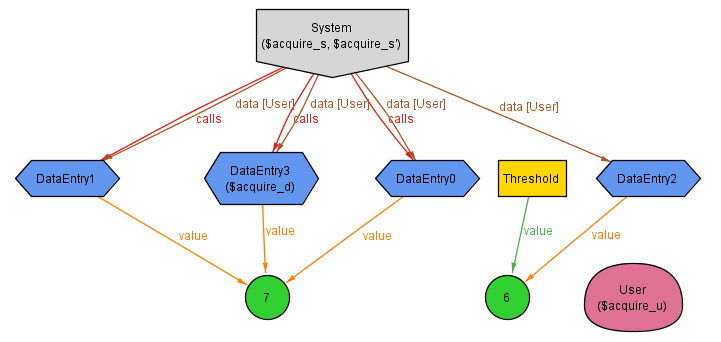
\includegraphics[width=\textwidth]{img/alloy/alloy_acquire.png}
    \caption{Acquisition of a new data entry that may trigger a SOS call}
    \label{fig:alloy_acquire}
  \end{figure}

  \begin{figure}[h!]
    \centering
    \hspace*{-1.5cm}
    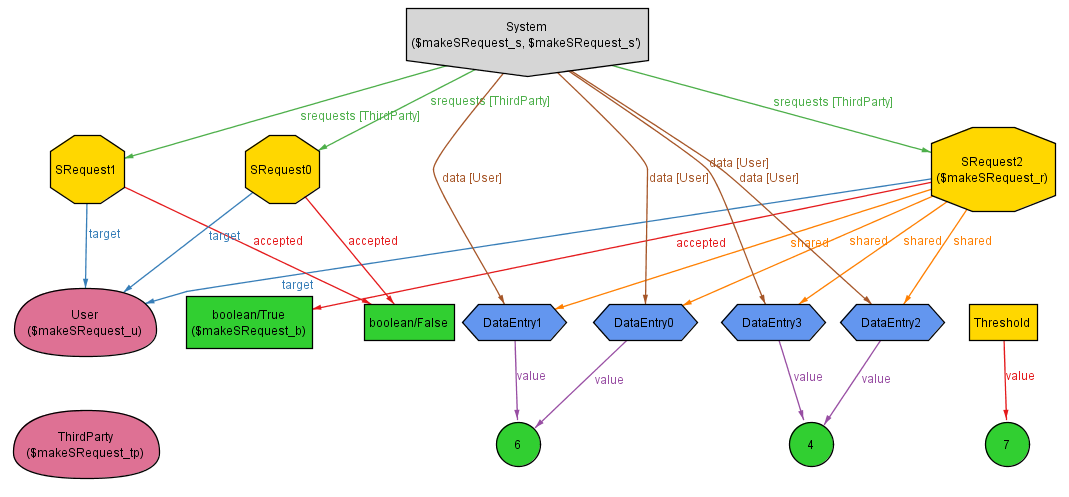
\includegraphics[width=1.15\textwidth]{img/alloy/alloy_srequest.png}
    \caption{Single user requests that may be accepted or refused by users}
    \label{fig:alloy_srequest}
  \end{figure}

  \begin{figure}[h!]
    \centering
    \hspace*{-0cm}
    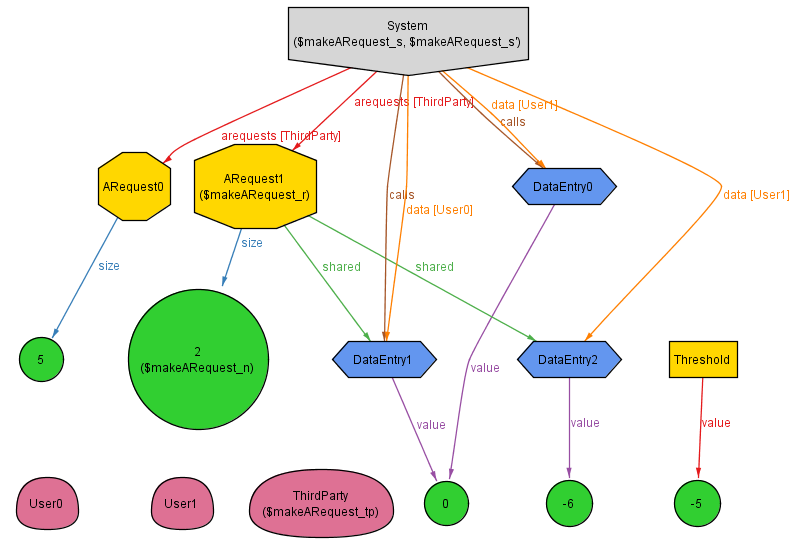
\includegraphics[width=\textwidth]{img/alloy/alloy_arequest.png}
    \caption{Anonymous group requests that may be accepted or refused by the system}
    \label{fig:alloy_arequest}
  \end{figure}

  \begin{figure}[h!]
    \centering
    \hspace*{-0cm}
    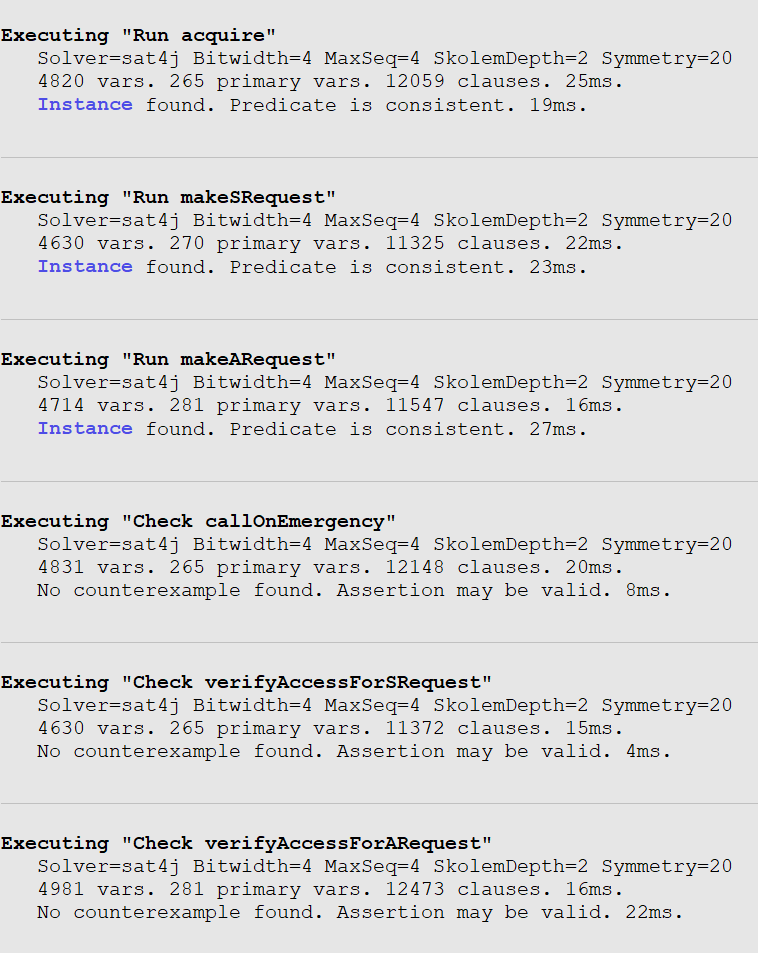
\includegraphics[width=\textwidth]{img/alloy/alloy_check.png}
    \caption{Model validation}
    \label{fig:alloy_check}
  \end{figure}

\clearpage
\section{Graphics}
\label{sec:graph}

\subsection{Use cases Diagram}



\subsubsection{Sign In}

\begin{figure}[h!]

\centering

\hspace*{-2.5cm}
\includegraphics[scale=0.7]{img/Sign_In.png}

%\caption{---}

 \label{fig:use_case_signin}

 \end{figure}

\clearpage


\subsubsection{Exploit app functionalities}



%hspace*{} before the figure and the figure must be immediately after the hspace* otherwise the system doesn't recognize it

\begin{figure}[h!]

\centering

\hspace*{-2.5cm}
\includegraphics[scale=0.7]{img/Normal_Behaviour.png}

%\caption{---}

  \label{fig:use_case_normalbehaviour}

 \end{figure}
\clearpage
\documentclass[../DD0.tex]{subfiles}

\newcommand{\addHours}[4]{#1 & #2 & #3 & #4 \\\hline}

\begin{document}

\section*{Effort spent}
\label{sec:effort}
  \begin{table}[h!]
  \centering
  \begin{tabularx}{\linewidth}{|l|c|c|X|Xl}
    \hline
    \textbf{Date}  & \textbf{Archetti Alberto} & \textbf{Carminati Fabio} & \textbf{Activity} \\ \hline
    \addHours{12/11/2018}{1}{1}{Introduction sketch}
    \addHours{24/11/2018}{}{6}{User Interface Design}
    \addHours{24/11/2018}{3}{}{High-level components}
    \addHours{25/11/2018}{2}{}{Application Server subcomponents}
    \addHours{26/11/2018}{}{5}{Architectural Design}
    \addHours{27/11/2018}{2}{}{Component interfaces}
    \addHours{27/11/2018}{}{3}{Requirement Traceability}
    \addHours{28/11/2018}{}{1}{Requirement Traceability}
    \addHours{30/11/2018}{1}{1}{High-level components}
    \addHours{1/12/2018}{6}{}{Update sequence diagrams and component interfaces; added component diagram}
    \addHours{2/12/2018}{5}{1}{Architectural styles and patterns, UI, traceability}
    \addHours{3/12/2018}{}{3}{Update sequence diagrams and interfaces}
    \addHours{4/12/2018}{3}{3}{Deployment, integration and testing}
  \end{tabularx}
\end{table}

\end{document}

\clearpage
\begin{thebibliography}{9}
  \bibitem{assignment} Mandatory Project Assignment AY 2018-2019

  \bibitem{ieee830} IEEE 830-1993 - IEEE Recommended Practice for Software Requirements Specifications

  \bibitem{ieee29148} ISO/IEC/IEEE 29148 - Systems and software engineering — Life cycle processes — Requirements engineering

  \bibitem{wereabledata} Collection and Processing of Data from Wrist Wearable Devices in Heterogeneous and Multiple-User Scenarios\\
  \texttt{https://www.ncbi.nlm.nih.gov/pmc/articles/PMC5038811/}

  \bibitem{sensors} Wearable Devices in Medical Internet of Things: Scientific Research and Commercially Available Devices\\
  \texttt{https://www.ncbi.nlm.nih.gov/pmc/articles/PMC5334130/}

  \bibitem{googlefitapi} Google Fit API\\
  \texttt{https://developers.google.com/fit/overview}

  \bibitem{paypal} PayPal API\\
  \texttt{https://developer.paypal.com/docs/}

  \bibitem{sos} RapidSOS Emergency API\\
  \texttt{https://info.rapidsos.com/blog/product-spotlight-rapidsos-emergency-api}

  \bibitem{slides}
  Slides of the course by Prof. Di Nitto\\
  \texttt{https://beep.metid.polimi.it/}

  %\bibitem{latexcompanion}
  %Michel Goossens, Frank Mittelbach, and Alexander Samarin.
  %\textit{The \LaTeX\ Companion}.
  %Addison-Wesley, Reading, Massachusetts, 1993.

  %\bibitem{einstein}
  %Albert Einstein.
  %\textit{Zur Elektrodynamik bewegter K{\"o}rper}. (German)
  %[\textit{On the electrodynamics of moving bodies}].
  %Annalen der Physik, 322(10):891–921, 1905.
\end{thebibliography}

\end{document}
